%% LyX 2.1.4 created this file.  For more info, see http://www.lyx.org/.
%% Do not edit unless you really know what you are doing.
\documentclass[english]{article}
\usepackage[T1]{fontenc}
\usepackage[latin9]{inputenc}
\usepackage{geometry}
\geometry{verbose,tmargin=3cm,bmargin=3cm,lmargin=3cm,rmargin=3cm}
\usepackage{color}
\usepackage{babel}
\usepackage{float}
\usepackage{amsmath}
\usepackage{amsthm}
\usepackage{graphicx}
\usepackage[unicode=true,pdfusetitle,
 bookmarks=true,bookmarksnumbered=true,bookmarksopen=true,bookmarksopenlevel=10,
 breaklinks=true,pdfborder={0 0 1},backref=false,colorlinks=true]
 {hyperref}
\hypersetup{
 linkcolor=blue, urlcolor=blue}

\makeatletter
%%%%%%%%%%%%%%%%%%%%%%%%%%%%%% Textclass specific LaTeX commands.
\numberwithin{equation}{section}
\numberwithin{figure}{section}

\makeatother

\usepackage{listings}
\renewcommand{\lstlistingname}{Listing}

\begin{document}

\author{bTactic - open source \& cloud solutions\\
\href{http://www.btactic.com}{http://www.btactic.com}}


\title{bSmtp zimlet - Admin manual}

\maketitle
\tableofcontents{}


\section{\label{sec:Instal=0000B7lar-el-Zimlet}Install zimlet}

To install from the server zimlet have to open a terminal with the
Zimbra server, and run the following commands:

\begin{lstlisting}[tabsize=4,frame=single]
$ su - zimbra
$ zmzimletctl deploy <path to file com_btactic_bsmtp.zip>
\end{lstlisting}
To install the zimlet from the terminal have to have previously downloaded
the zip containing the zimlet on the server.\\
\\
This is an example of the result of executing the commands described
above:

\begin{lstlisting}[tabsize=4,frame=single]
$ zmzimletctl deploy /home/btactic/com_btactic_bsmtp.zip
[] INFO: Deploying Zimlet com_btactic_bsmtp in LDAP.
[] INFO: Installing Zimlet com_btactic_bsmtp on this host.
[] INFO: Upgrading Zimlet com_btactic_bsmtp to 1.0
[] INFO: Adding Zimlet com_btactic_bsmtp to COS default
[] INFO: Enabling Zimlet com_btactic_bsmtp
\end{lstlisting}



\section{Post instalation}

For the zimlet function properly have to run the following commands
from the terminal server Zimbra:

\begin{lstlisting}[tabsize=4,frame=single]
$ su - zimbra
$ zmprov modifyServer $(zmhostname) zimbraZimletJspEnabled TRUE
$ zmcontrol restart
\end{lstlisting}
In the case of having a multi-server installation of Zimbra you must
be run on all mailbox servers.


\section{\label{sec:3 Activar i desactivar el Zimlet}Enable/disable zimlet}

To modify zimlet status (enable / disable) must access configuration
zimlets. Let the process to follow:
\begin{enumerate}
\item As shown in figure \ref{fig:Pas 1} The first step is to enter the
Zimbra Administration Console and then \textbf{\emph{Configure}}.


\begin{figure}[H]
\begin{centering}
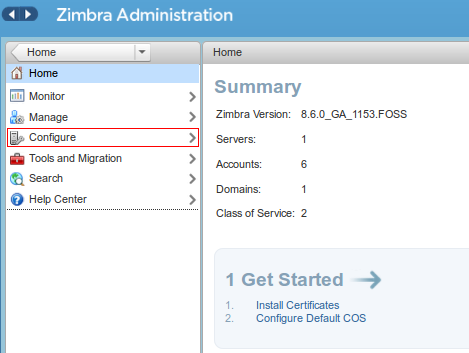
\includegraphics[clip,scale=0.5]{screenshots_admin_en/Step1-1}
\par\end{centering}

\caption{\label{fig:Pas 1}Starter window of admin console }
\end{figure}


\item Then go to \textbf{\emph{Zimlets }}(see figure \ref{fig:Pas 2}).


\begin{figure}[H]
\begin{centering}
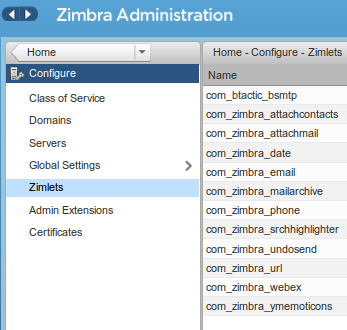
\includegraphics[clip,scale=0.5]{screenshots_admin_en/Step1-2}
\par\end{centering}

\caption{\label{fig:Pas 2}Configuration Panel, section \textbf{\emph{Zimlets}}}
\end{figure}


\end{enumerate}
Once we are in the configuration panel Zimlets, we have to click with
the right mouse button over\textbf{\emph{ com\_btactic\_bsmtp}}. In
the menu displayed select \textbf{\emph{Toggle Status}} (see figure
\ref{fig:Activar i desactivar zimlet}).\\
\\
This procedure caused the state zimlet pass enable to disable or vice
versa. We can know what state the zimlet by looking at the \emph{Status}
column.\\
\\
For the zimlet available state must be \textbf{\emph{Enabled}}, otherwise
(state \textbf{\emph{Disabled}}) is not available.

\begin{figure}[H]
\begin{centering}
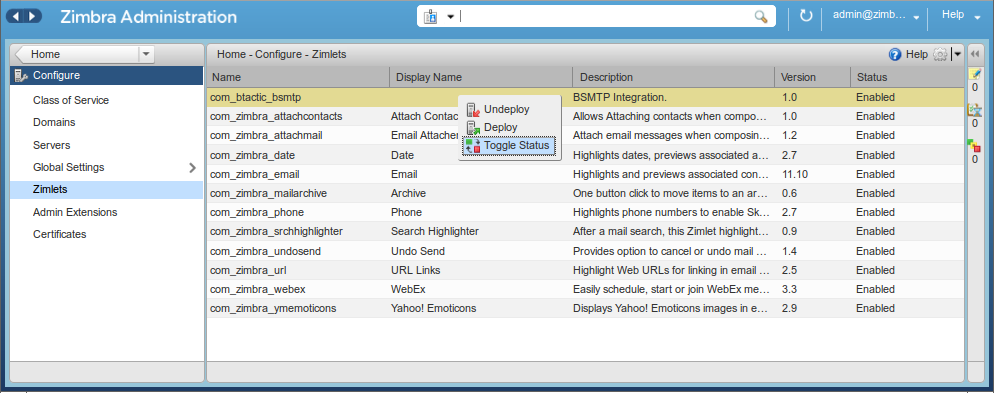
\includegraphics[clip,scale=0.5]{screenshots_admin_en/Step3-1}
\par\end{centering}

\caption{\label{fig:Activar i desactivar zimlet}Enable / disable zimlet}
\end{figure}



\section{Habilitar el zimlet en la clase de servicio del usuario}

To enable zimlet in the class of service user have to enter the management
console, Configure tab (more details in step 1 of \ref{sec:3 Activar i desactivar el Zimlet})
and once there, we have to follow the steps below:
\begin{enumerate}
\item On the left menu click\textbf{\emph{ Class of Service}} and select
the kind of service we want to have zimlet (see Figure \ref{fig:Configuraci=0000F3 classe de servei}).


\begin{figure}[H]
\begin{centering}
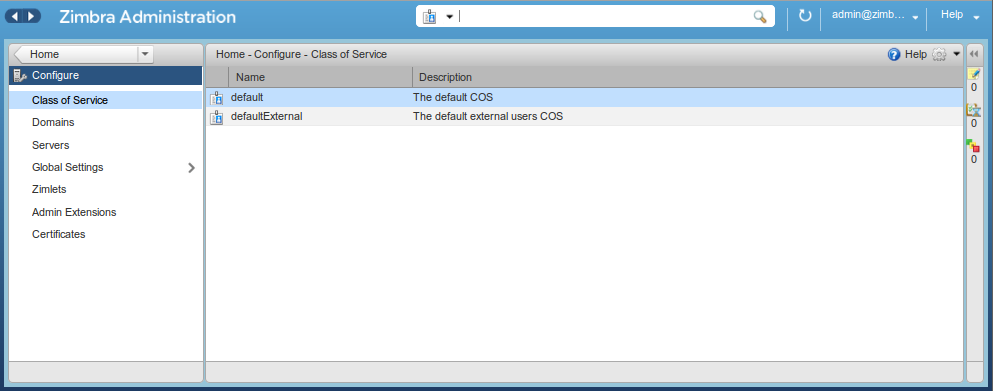
\includegraphics[clip,scale=0.5]{screenshots_admin_en/Step4-1}
\par\end{centering}

\caption{\label{fig:Configuraci=0000F3 classe de servei}Configuration \textbf{\emph{Class
of Service}}}
\end{figure}


\item Once we are in the kind of service we want to edit, we need to click
the icon at the top right of the screen and select the option\textbf{\emph{
Edit}}\emph{ }(see figure \ref{fig:Editar classe de servei})\emph{.}


\begin{figure}[H]
\begin{centering}
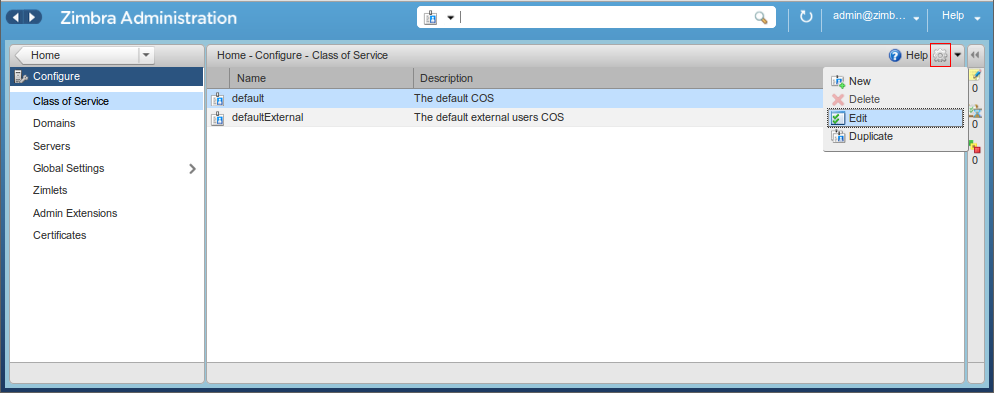
\includegraphics[clip,scale=0.5]{screenshots_admin_en/Step4-2}
\par\end{centering}

\caption{\label{fig:Editar classe de servei}Edit \textbf{\emph{Class of Service}}}
\end{figure}


\item Once we find in shaping the kind of service we want to edit, we have
to go to \textbf{\emph{Zimlets}} panel section on the left and once
there edit the configuration \textbf{\emph{com\_btactic\_bsmtp}} of
the following this rules: 

\begin{itemize}
\item \textbf{Mandatory }zimlet will activate and cause the zimlet invisible
on the preference of the Web client. Therefore, the user can not disable
the zimlet.
\item \textbf{Enabled} and \textbf{disabled}\textbf{\emph{ }}only define
the default status zimlet. Users can enable and disable it.
\end{itemize}

See figure \ref{fig:Configuraci=0000F3 dels Zimlets a la classe de servei}.


\begin{figure}[H]
\begin{centering}
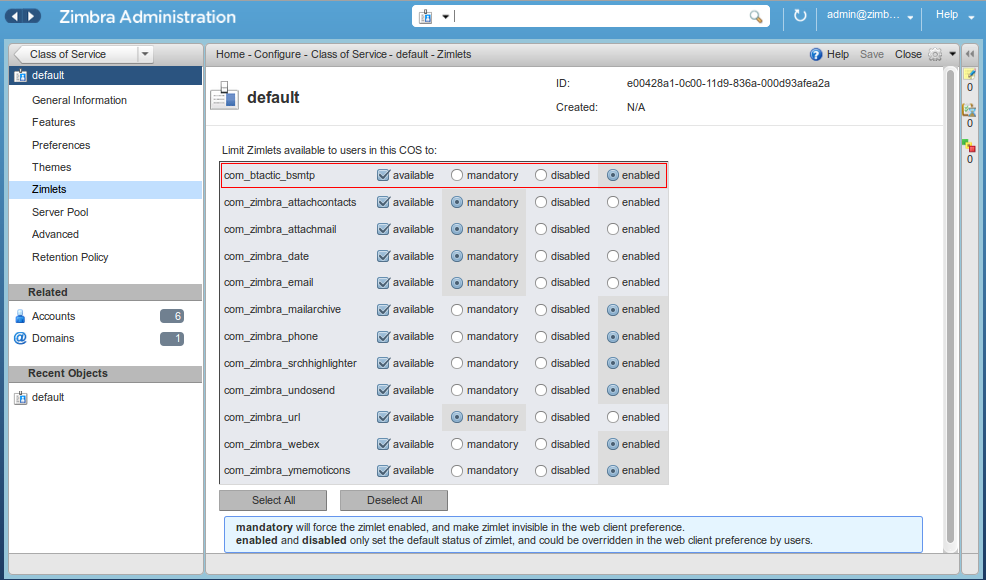
\includegraphics[clip,scale=0.5]{screenshots_admin_en/Step4-3}
\par\end{centering}

\caption{\label{fig:Configuraci=0000F3 dels Zimlets a la classe de servei}Configuration
zimlets in \textbf{\emph{Class of Service}}}
\end{figure}


\end{enumerate}

\section{Source code zimlet}

The source code distributions are available zimlet\href{https://github.com/btactic/bsmtp}{https://github.com/btactic/bsmtp}
\end{document}
